\documentclass[lettersize,journal]{IEEEtran}
\usepackage{amsmath,amsfonts}
\usepackage{algorithmic}
\usepackage{algorithm}
\usepackage{array}
\usepackage[caption=false,font=normalsize,labelfont=sf,textfont=sf]{subfig}
\usepackage{textcomp}
\usepackage{stfloats}
\usepackage{url}
\usepackage{verbatim}
\usepackage{graphicx}
\usepackage{cite}
\hyphenation{op-tical net-works semi-conduc-tor IEEE-Xplore}
% updated with editorial comments 8/9/2021

\usepackage{caption}
\usepackage{subcaption}
\usepackage{hyperref}
\hypersetup{
    colorlinks=true,
    linkcolor=blue,
    citecolor=blue,
    filecolor=magenta,      
    urlcolor=cyan,
    pdftitle={Overleaf Example},
    pdfpagemode=FullScreen,
    }

\begin{document}

\title{Significance of Image Pre-processing in Computer Vision Based Fire Detection, A Review}

\author{Ashwin Rajesh
% <-this % stops a space
\thanks{This paper was produced by the IEEE Publication Technology Group. They are in Piscataway, NJ.}% <-this % stops a space
\thanks{Manuscript received April 19, 2021; revised August 16, 2021.}}

% The paper headers
\markboth{Journal of \LaTeX\ Class Files,~Vol.~14, No.~8, August~2021}%
{Shell \MakeLowercase{\textit{et al.}}: A Sample Article Using IEEEtran.cls for IEEE Journals}

\IEEEpubid{0000--0000/00\$00.00~\copyright~2021 IEEE}
% Remember, if you use this you must call \IEEEpubidadjcol in the second
% column for its text to clear the IEEEpubid mark.

\maketitle

\begin{abstract}
        This document describes the most common article elements and how to use the IEEEtran class with \LaTeX \ to produce files that are suitable for submission to the IEEE.  IEEEtran can produce conference, journal, and technical note (correspondence) papers with a suitable choice of class options. 
\end{abstract}

% \begin{IEEEkeywords}
% Article submission, IEEE, IEEEtran, journal, \LaTeX, paper, template, typesetting.
% \end{IEEEkeywords}

\section{Introduction}
\IEEEPARstart{W}{ildfires} pose a significant threat to humans, wildlife and the
environment alike. Left unchecked, A wildfire can spread rapidly causing
large scale destruction to forests \& infrastructure, as well as
releasing large amounts of pollutants into the atmosphere.

Studies have uncovered very strong associations of wildfire smoke with cardiovascular mortality, asthma hospitalisation and further susceptibility to cardiopulmonary effects in elderly adults.
The risk of premature death and respiratory morbidity in the general population are also increased due to wildfilre smoke \cite{wildfirehealth}.
Furthermore, ambient air pollution caused by wildfire smoke has been studied to have adverse affects on children, as a result of their developing lungs and inferior nasal deposition \cite{wildfirechildren}.
Breathing in wildfire smoke can cause chest pain and tightness, trouble breathing, diziness and other symptoms in children \cite{wildfirefactsheet}.

Wildfires have been consuming increasingly large areas of forest globally in recent years, causing vast amounts of damage to the environment in the form of water \& air pollution, climate change and destruction of flora and fauna.
Sediment exports in water bodies reportedly may increase by up to 1459 times the unburned amount, drastically degrading water quality in the affected areas. \cite{wildfirewater}.
Emissions of airborne particulate matter from wildfires can significant cause significant disruptions to air pollution mitigation targets set by legislation. \cite{wildfireair} shows that in high-fire seasons, pollution levels can reach dangerous levels despite aggressive reduction of anthropogenic emissions.
An estimated 97000 km\textsuperscript{2} of vegetation was burned in the 2019-2020 Australian bushfires, causing devastating damage to wildlife habitat, with many belonging to species listed at threatened to extinction \cite{wildfireveg}.

Evidently, It has become increasingly crucial to detect wildfires as early as possible to minimize damage to humans and the environment. Current methods of wildfire detection involve three main approaches:
\begin{enumerate}
\item{Terrestrial sensor nodes, which may be placed at fire-prone locations to detect wildfires through environmental readings.}
\item{UAVs can be employed to scan large forest areas and inaccessible terrain.}
\item{Satellite based systems can cover vast areas of land and determine the extent and direction of wildfires.}
\end{enumerate}

Despite the various classifications of technologies within wildfire
detection, advancements in computer vision object detection has spurred
use in terrestrial, aerial as well as satellite systems. \cite{satellite}
explores the feasibility of space-borne fire detection using onboard
computer vision to rapidly generate alerts. The traditional method of
downloading image data from satellites has too much latency for
time-sensitive applications such as fire detection. By examining
performance of hardware accelerators for edge computing such as Nvidia
Jetson and Movidius Myriad 2, the report found that AI inference
on-board the satellite is possible in terms of performance as well as
power consumption, allowing for low latency detection of wildfires.
\cite{uavai} details methods to optimise Deep Learning to deal with UAV
limitations such as image degredation, small fire size \& background
complexity. By combining EfficientNet-B5, vision transformers and
EfficientSeg convolutional model, an accuracy of 85.12\% was obtained,
outperforming many state-of-the-art models. \cite{wsnyolo} proposes a low
cost WSN fire detection approach based on YOLO object detection models.
The system, named SDFS was trained on a dataset of 26,520 images and
achieved a high precision rate of 97.1\% for smoke and fire
classification.
\IEEEpubidadjcol

Due to the importance of computer vision based object detection in
wildfire detection, it is imperative that they are as accurate as
possible. There are many different techniques to improve the performance
of neural networks. Transfer learning is the process of using a model
that has been pre-trained on a large dataset and further training and
fine tuning it to a specific task. \cite{transferlearning} studies the
impact of transfer learning on classification by comparing six differnet
pre-trained architectures. The models were trained using an open access
dataset of 3886 images and found that all six architectures were able to
achieve a testing accuracy of above 90\% despite a relatively small
training dataset. Augmenting data with synthetically generated samples
investigated by \cite{augment} found that inserting data-space
transformations such as warped images provided improved performance and
reduced overfitting. \cite{prepfire} proposed an image pre-processing
pipeline using advanced techniques such as HSV filters and corner
detection to assist models with classification by eliminating unwanted
noise in images. This method has observed to improve fire detection
accuracy by 5.5\% and smoke detection by 6\% in object detection models.

% ISSUES
% come around to edge computing CV problem here
However, detecting smoke and fire can prove challenging to a neural network model for a variety of reasons.
Uneven and dim lighting conditions can pose substantial difficulties while detecting smoke edges in an image.
The inconsistent shape and colour of fire as well as smoke can further cause complications.
Xin et al. \cite{resnetsmoke} Employs the use of a deep ResNet architecture in order to tackle this issue.
Accurately and consistently detecting smoke, as a result, tends to require deeper models that are capable of learning complex features.
Wildfire detection is often performed in remote terrestrial regions, aerially or from space, which will limit the computational power available for running neural networks.
Additionally, the network must maintain real-time inference, as latency is critical in detecting fires as early as possible.
These factors make larger complex neural networks suboptimal for wildfire detection.
Therefore, a solution to real-time smoke detection that can be powered by low-specification edge computing devices such as a Raspberry Pi must be explored.

% ADDRESSING THE PROBLEM
This report aims to explore different methods employed in improving the
performance and efficiency of wildfire detection systems, with a focus
on computer vision based fire detection using Convolutional Neural
Networks (CNNs). Fire and smoke detection is carried out through a variety of
mediums, such as terrestrial sensor nodes, UAV scanning and satellite
based approaches. Observing the literature, it is apparent that computer
vision plays a significant role in all systems, Making it important to
maximise their efficiency and accuracy. Furthermore, it is important to
optimise such systems to run on low-powered edge computing devices,
which are currently used to detect wildfires. To this end, a multitude
of image preprocessing filters relevant to smoke detection were explored. 
A pipeline of processing that involves Dark Channel Prior in combination with smoke edge detection with Sobel kernels is proposed and benchmarked in this report. 
The proposed dark channel prior + edge detection algorithm
aims to improve on existing methods of smoke preprocessing using DCP
detailed in \cite{prepfire}. Specifically, false positives due to high
light intensity artifacts in the image such as the sky are significantly
mitigated, thanks to edge detection filters revealing characteristics
that are unique to smoke.

The benchmarks are carried out on a Raspberry Pi 4B, to
similate low-powered edge computing hardware that is consistently used
in terrestrial, UAV and satellite systems. Large deep-learning networks
are unviable on these systems due to the high computational intensity,
while models with reduced parameters are more efficient but suffer from
less accurate inference. The preprocessing pipeline aims to improve the
accuracy of lightweight models by highlighting important features in
fire and smoke, while reducing unwanted noise in the image.
To this end, a YOLOv8 nano model is trained on an open source Wildfire Smoke Detection dataset \cite{yolov8}.
This model is compared with another model that has been trained on the exact same dataset, but with the smoke enhancing preprocessing pipeline stated above.

%Furthermore, an improved system for early smoke detection is
%investigated. 
% This paper contributes a benchmark of different pre-processing filters
%and algorithms to uncover insights on an ideal pipeline for wildfire
%detection, using metrics such as speed, power consumption and model
%accuracy.

\section{Literature Review}


\begin{figure}
        \centering
        \includegraphics[width=2.5in]{sensornode.png}
        \caption{Basic operation of WSNs. Images sourced from Creative Commons,
        following the guidelines on Attribution 3.0 Unported, CC By 3.0}
\end{figure}

\begin{figure}
        \centering
        \includegraphics[width=2.5in]{wildfire_satellite.png}
        \caption{Satellite Based Wildfire Detection}
\end{figure}

Edge computing sensor nodes can be placed at high risk locations that
can monitor temperature, humidity and other characteristics of air in
the surrounding area. These systems generally use a microcontroller to
operate sensors, relying on solar cells for long-term power. By setting
up multiple such nodes in different areas forming a Wireless Sensor
Network (WSN), the collected sensor data may then be analyzed to
determine the locations of fire events \cite{MohapatraAnkita2022EWDT}.
More advance methods of data classification with the use of artificial
neural networks boast a high accuracy of \textgreater82\% with multiple
sensors \cite{wsnfire}. The low cost of WSN systems has made it an
increasingly popular choice for real-time monitoring of forest fires.
However, sensor nodes fail to be viable in some situations. Establishing
wireless communications for a WSN can prove challenging in rural or
untamed areas such as forests \cite{wsnyolo}. The sensor nodes may also
be prone to damage from the wildfire, needing to be replaced in order to
continue using the system.

UAVs have seen extensive research for this application, as they provide
valuable visual data which can be employed to carry out search and
rescue operations, save forest resources, help firefighters navigate
efficiently amoung numerous other enhancements. Rather than sending
ground crews to monitor hazardous environments, UAVs can drastically
reduce the risk to firefighting crews by remotely scanning large amounts
of dangerous forest area. However UAVs tend to perform poorly in harsh
weather conditions, have limited flight time and require a human
operator to have a visual line of sight \cite{uav}. These factors
combined with expensive operation costs severly limit the effectiveness
of UAVs in many circumstances.

Satellite-based fire detection can potentially offer significant
advantages over traditional methods due to the vast areas they can
monitor. The benefits and limitations of these systems largely depend on
the satellite's orbit. Satellites in Sun-Synchronous Orbit (SSO) provide
high spatial resolution but revisit the same location only after several
days, resulting in low temporal resolution. This delay makes SSO
satellites less effective for real-time wildfire detection
\cite{satellite}. In contrast, Geostationary Earth Orbit (GEO) satellites
remain fixed over the same region, as their orbital period matches
Earth's rotation. Equipped with multispectral imaging sensors, GEO
satellites provide continuous monitoring, making them ideal for
detecting and tracking fires in real time.

\subsection{Image Pre-Processing Algorithms}

\subsubsection{HSV filter}

Hue, Saturation, Value (HSV) is a cylindrical-coordinate representation
of points in an RGB colour model. It is an alternative representation of
the RGB color model that intends to describe colors in a way that is
more aligned with human perception. Colour masks can be created by
setting upper and lower bounds within the HSV channels. This can then be
applied to an image to filter specific tones of colour. A study by
\cite{skinhsv} utilized HSV thresholding to detect human skin in an
image. The process achieved an impressive 99.587\% accuracy on natural
images under varying light conditions. \cite{prepfire} used a HSV filter
in addition to other preprocessing stages to isolate colours of fire in
an image to assist object detection models with inference, which
resulted in a 5.5\% increase in fire detection accuracy. The following
bounds were used to preprocess images in the paper:

\[\text{ RoI}_{\text{HSV(x,y) }} := \begin{cases}
        1, 20 < H(x,y) < 40 \\
        \text{ and }50 < S(x,y) < 255 \\
        \text{ and }50 < V(x,y) < 255 \\
        0, otherwise
\end{cases}\]

% \begin{figure}
%         \centering
%         \begin{subfigure}[b]{0.5\textwidth}
%                 \centering
%                 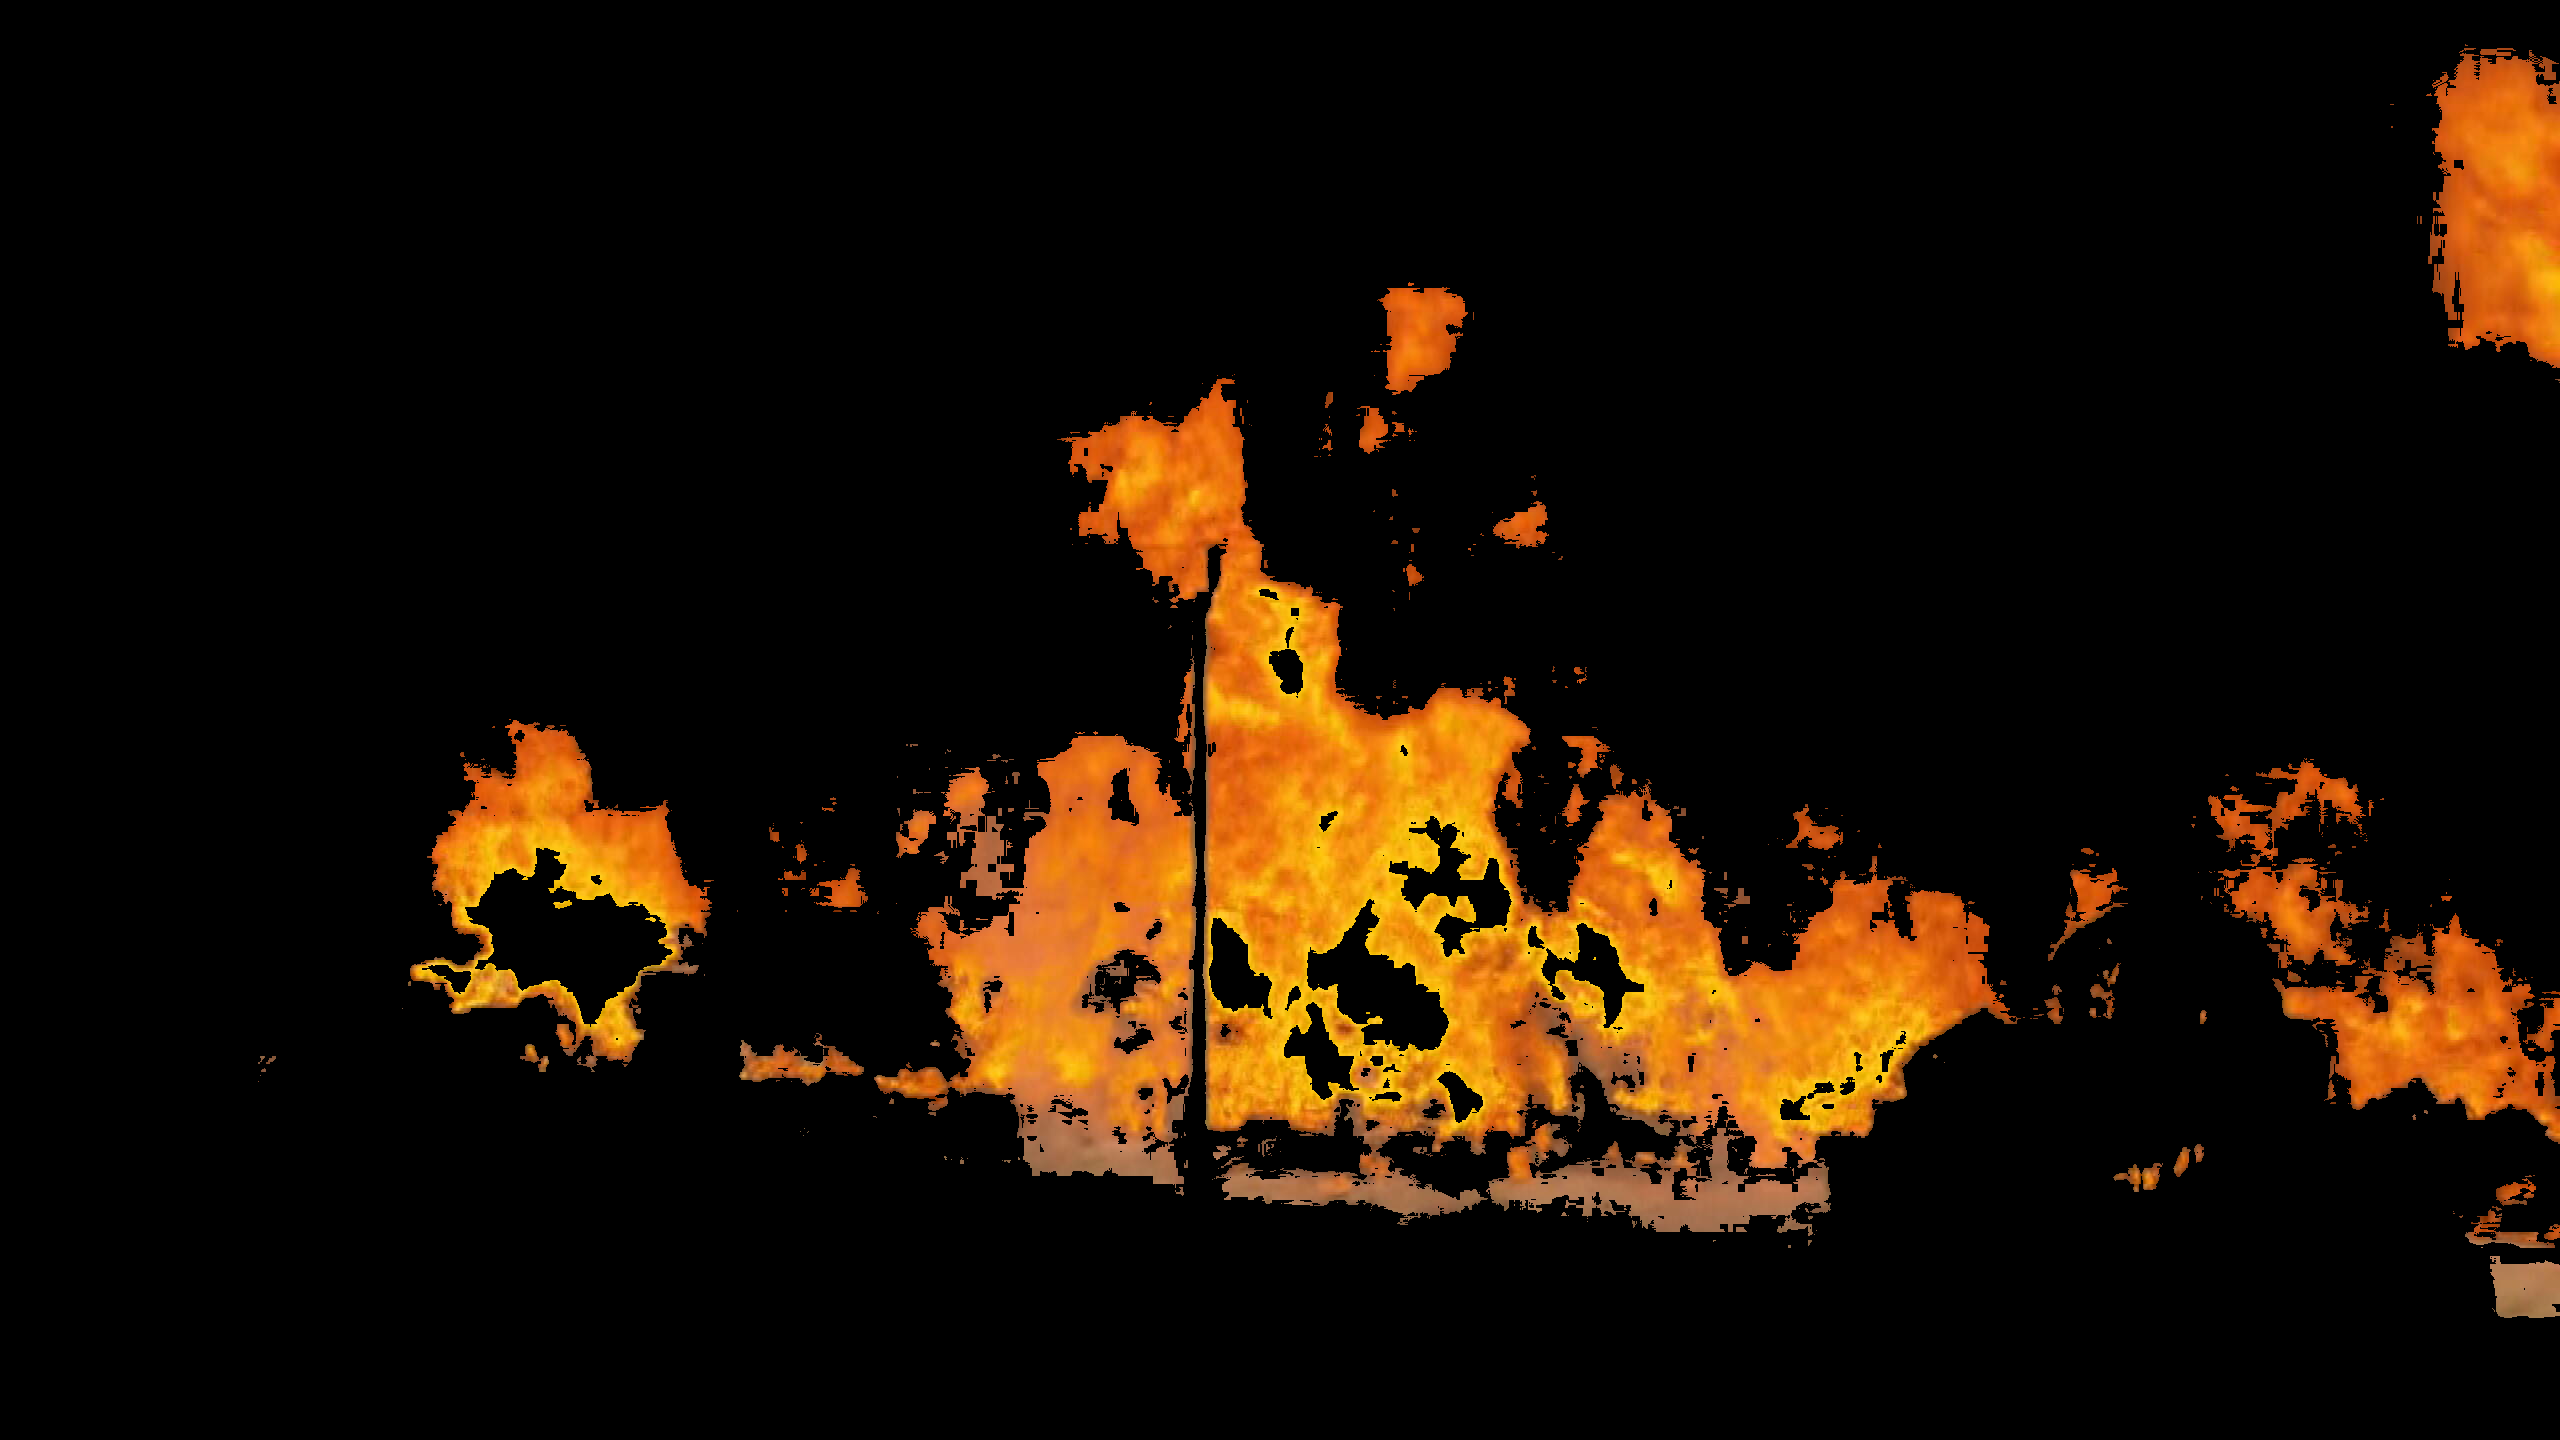
\includegraphics[width=\textwidth]{hsv_filter.png}
%                 \caption{$filtered image$}
%                 \label{fig:y equals x}
%         \end{subfigure}
%         \hfill
%         \begin{subfigure}[b]{0.5\textwidth}
%                 \centering
%                 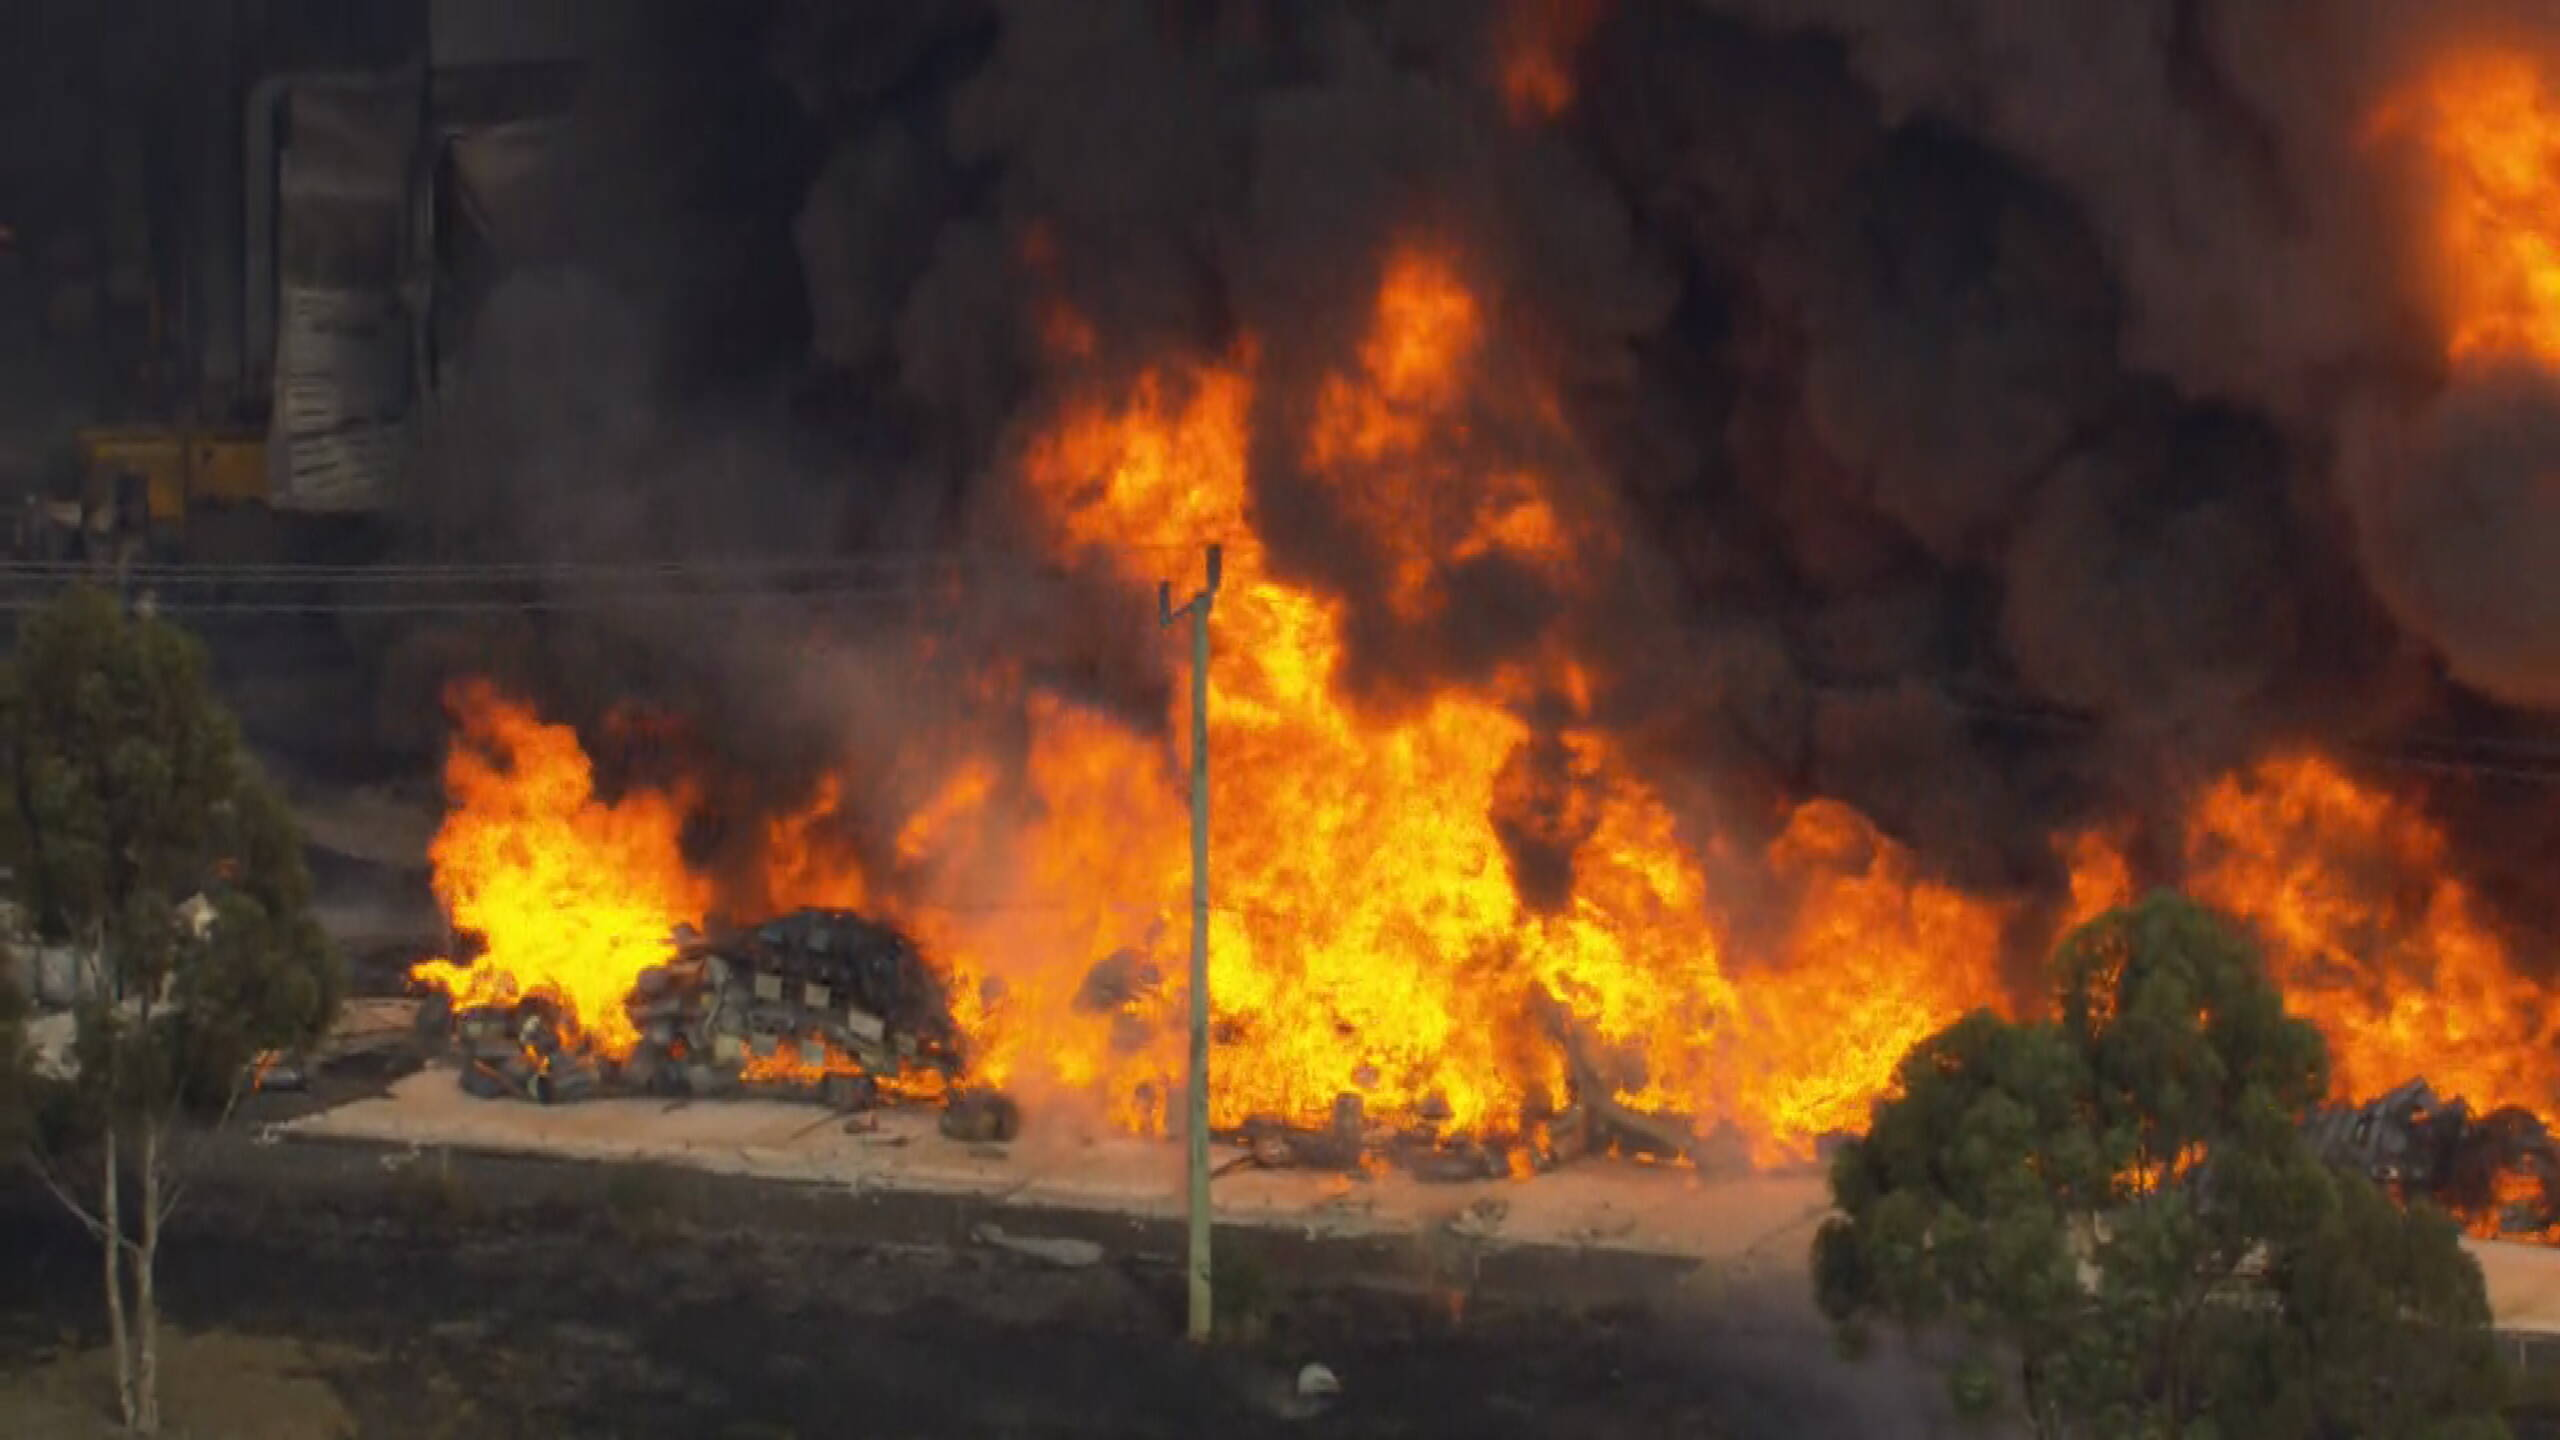
\includegraphics[width=\textwidth]{hsv_original.jpeg}
%                 \caption{$original image$}
%                 \label{fig:y equals x}
%         \end{subfigure}
%         \caption{Resulting Image after HSV mask}
% \end{figure}

\begin{figure*}[!t]
\centering
\subfloat[]{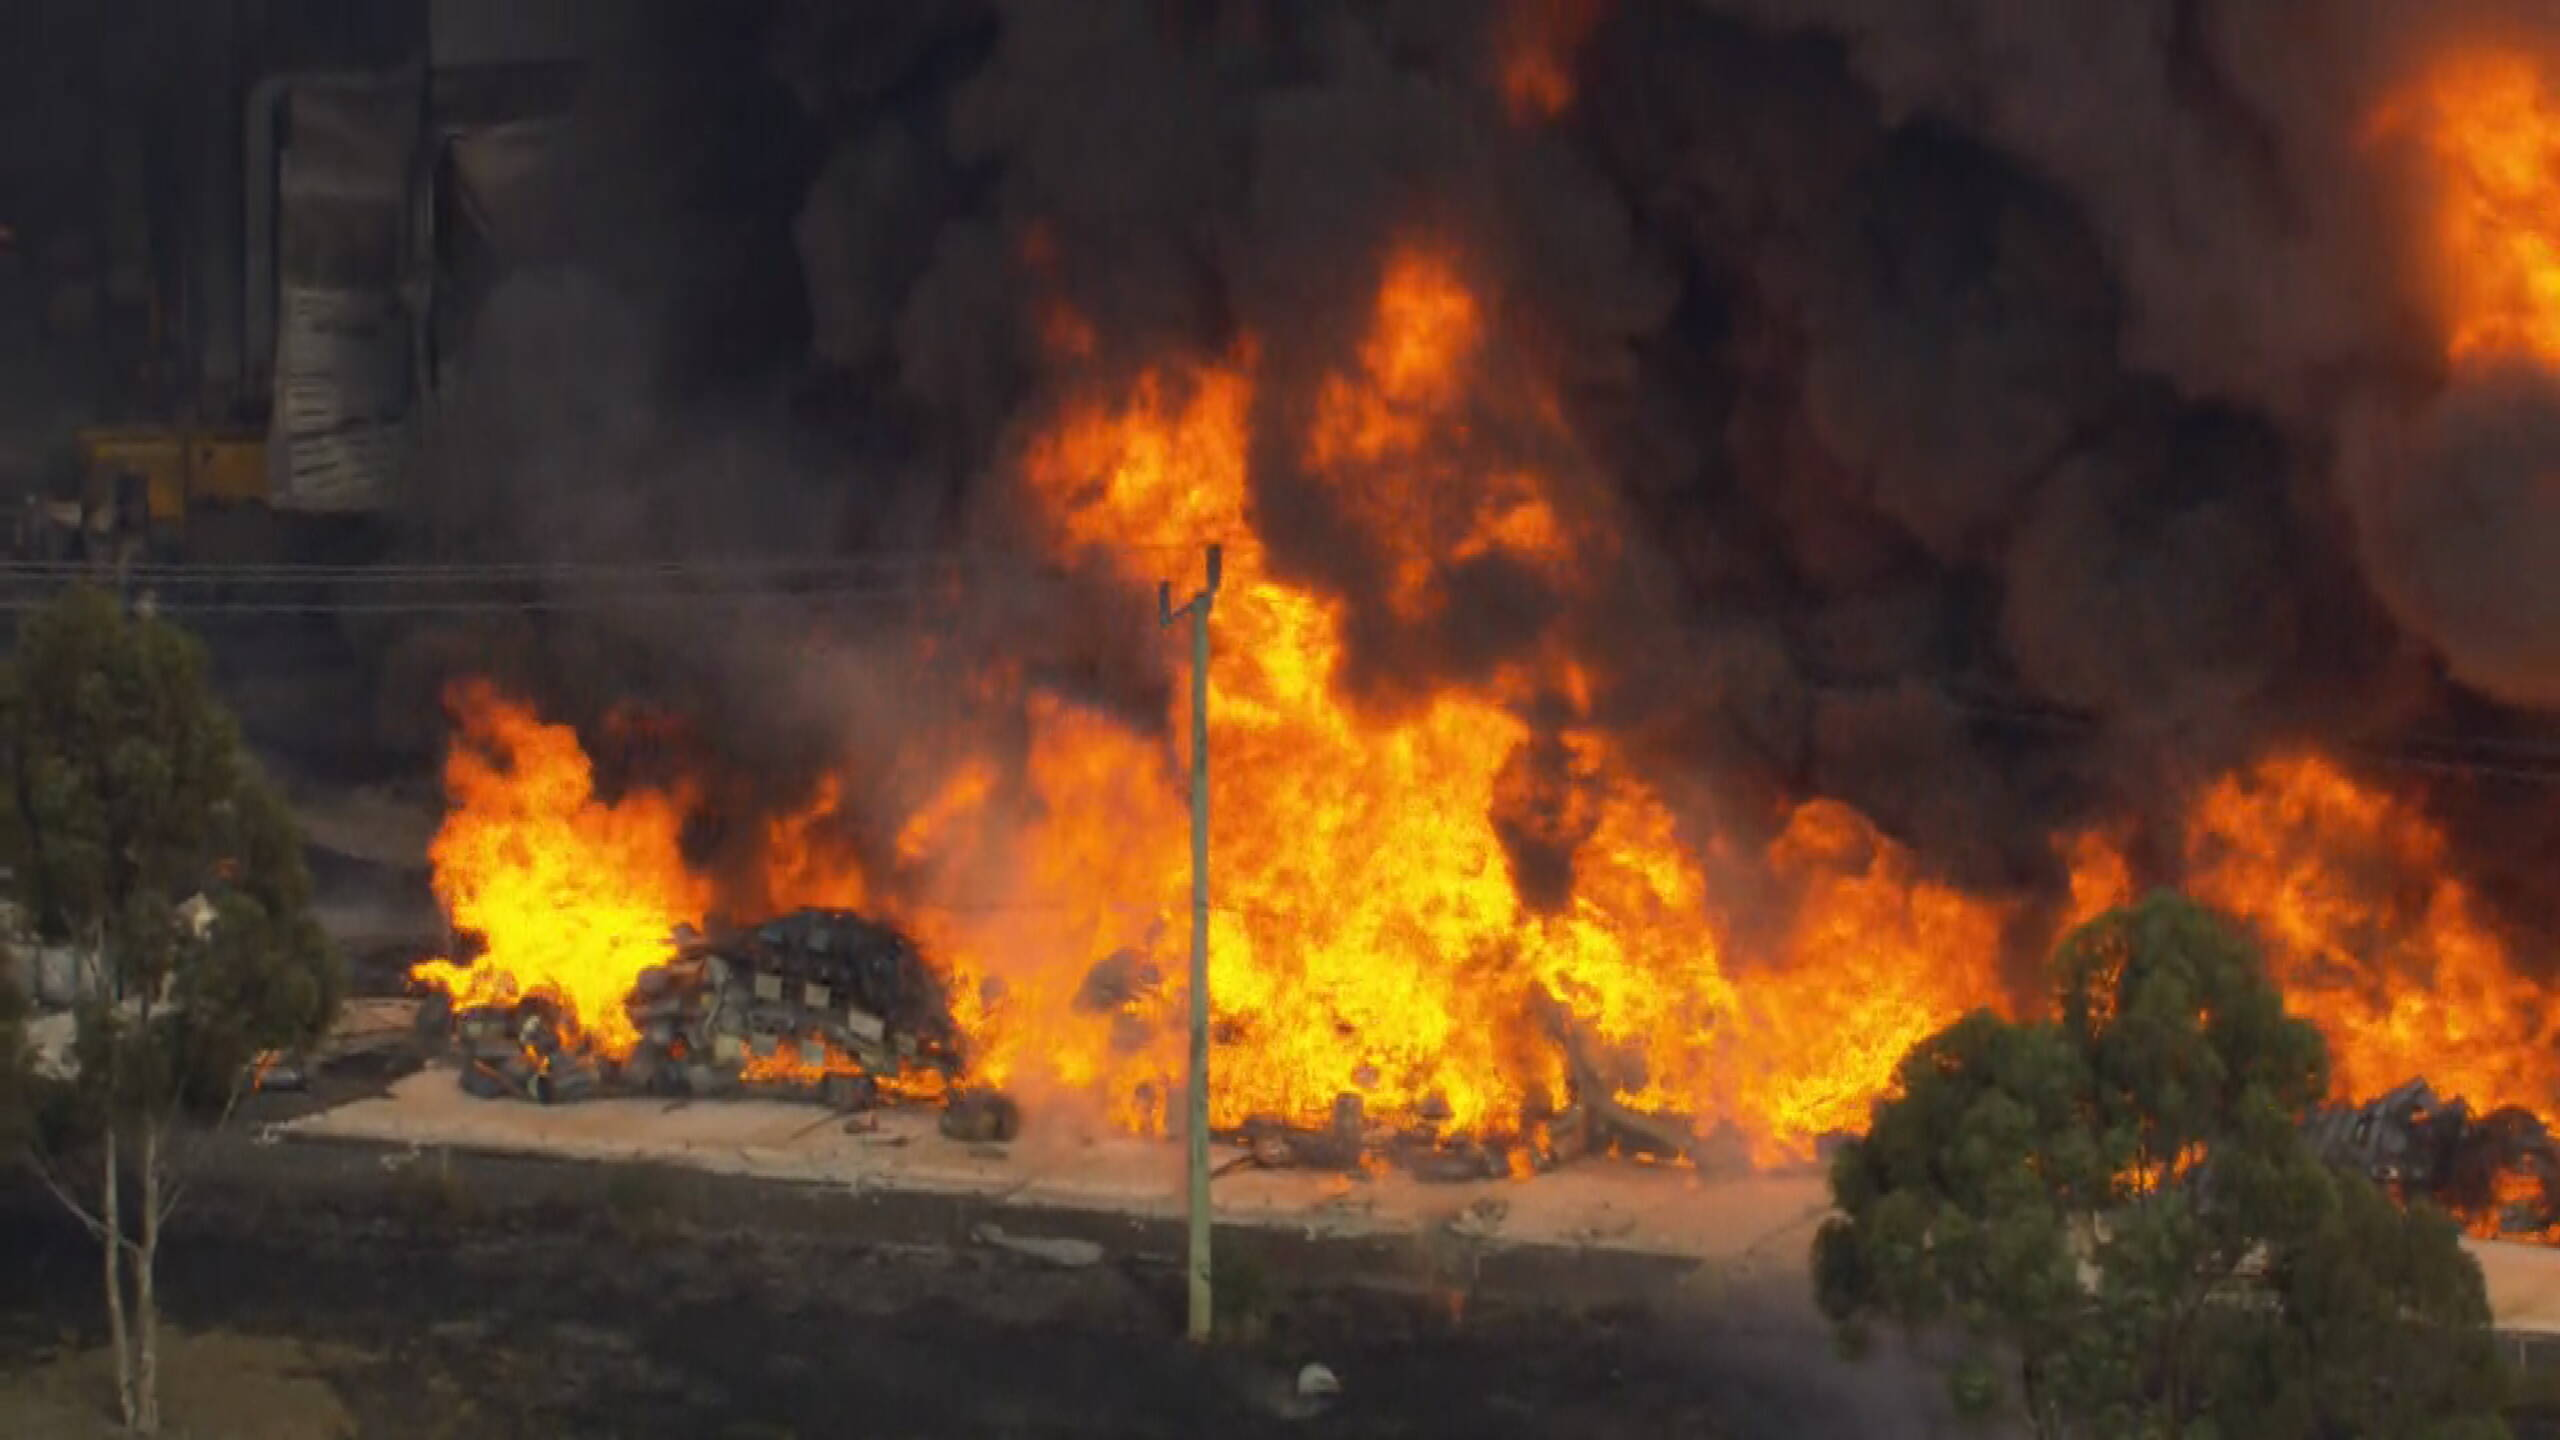
\includegraphics[width=2.5in]{hsv_original.jpeg}%
\label{hsv_orig}}
\hfil
\subfloat[]{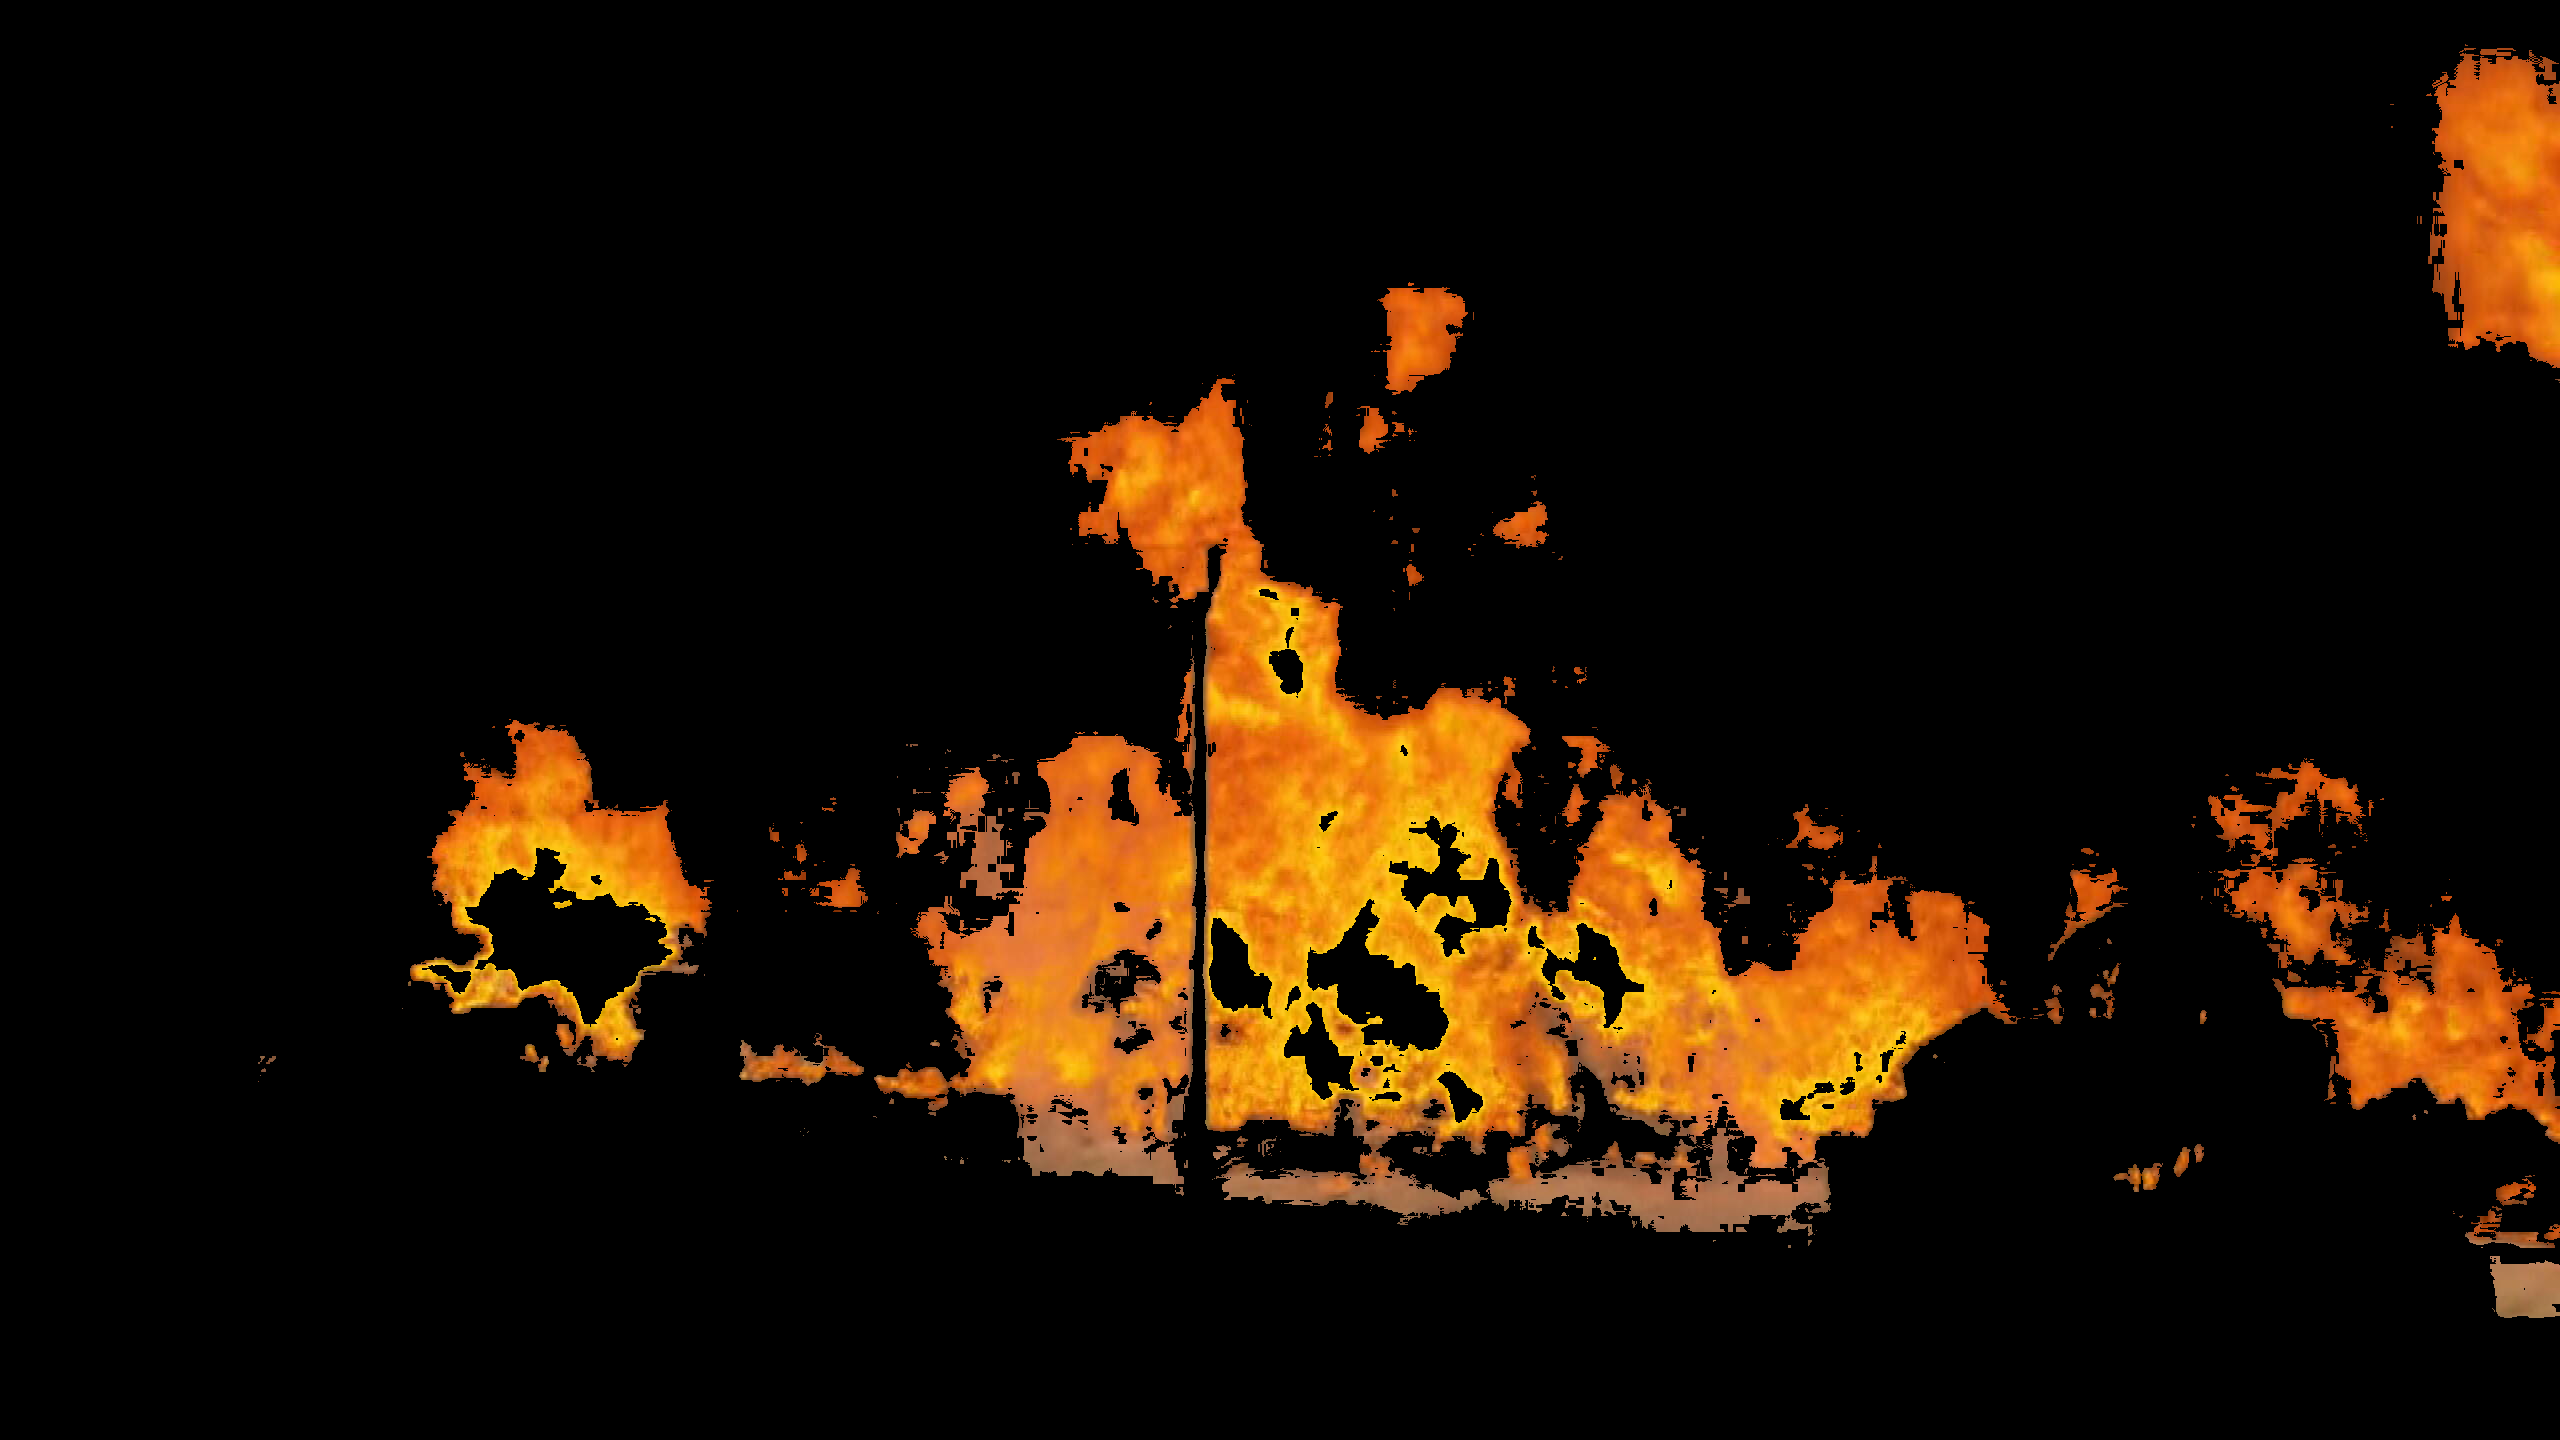
\includegraphics[width=2.5in]{hsv_filter.png}%
\label{hsv_filter}}
        \caption{Example of Image filtered using the described HSV mask. (a) Original image. (b) Filtered image.}
\label{hsvimg}
\end{figure*}


\subsubsection{Edge \& Contour Detection}

Edge detection involves identifying regions of an image where the
contrast between pixels changes dramatically. Capturing edges can be
used to reveal important properties in the image as these edges often
correspond to changes in depth, illumination, orientation or material.
Edge detection can be particularly useful in detecting fire, as it
uncovers data about positions of contours and contrasts where fire and
smoke could potentially exist. More specifically, method to use low edge
responses in an image region may be useful in differentiating between
smoke and sky. This method is explored further in this paper

Edge detection has seen use in many fields to extract valuable
information from visual data. \cite{covidsobel} aims to accurately detect
COVID-19 patients by using edge detection to improve detection accuracy
of a CNN on CT images of the lungs. The addition of sobel edge detection
to a CNN proved to be an effective approach, achieving an accuracy of
99.02\% on a custom dataset. \cite{edgesat} proposes an approach to
detect roads in satellite images using edge detection and
semantic-segmentation. The results showed accurate segmentation \& edge
detection even in complicated backgrounds. This shows the potential of
edge detection in satellite and UAV based systems, where small details
in an image are of significant importance.

A popular method of edge detection thanks to its computational
simplicity is the Sobel operator. The sobel filter involves convolving
the image with a specific kernel which calculates the gradient of the
image in x and y directions \cite{sobel}. For a given image, let us
consider a pixel region such as in figure \ref{pixregion}.

The figure shows the value in each cell is the brightness of the pixel in that
position within the image. In the region shown above, we can see that
the pixel brightness rapidly changes between the 2nd and 3rd columns,
which would be perceived as an edge by humans. We can then convolve the
gradient filter shown in figure \ref{gradfilter} over each pixel of the image.

Let us consider the pixel in the second column and second row as the
pixel currently being processed. Each value in the gradient filter is
multiplied with the corresponding pixel in the neighbouring 3x3 area
around our center pixel, and summed. In our example, this would output a
high value of 200, as our area of interest contains high intensity
pixels on the right and lower intensity on the left.

This process is repeated with every other pixel to produce the partial
derivative of the image in the x direction. By obtaining the y partial
derivative in a similar manner, we may combine the images to produce a
resultant image containing high absolute values near edges and a value
close to 0 everywhere else. The x and y gradients can be combined using
the following method:

\[G = \sqrt{G_{x}^{2} + G_{y}^{2}}\]

Where G is the positive magnitude of the intensity of an edge at that
pixel. Pixels with small edge response will have a value closer to 0
(black) while pixels around an edge will have a high value and appear
white. The effects of a sobel filter on an image can be seen in figure
\ref{sobelimg}, where most of the scenery and smoke
is covered in many white lines, while the small area of sky above is
almost completely dark.

\begin{figure}
        \centering
        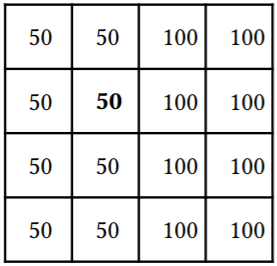
\includegraphics[width=1in]{sobel_pixels.png}
        \caption{Pixel region where numbers indicate brightness of the pixel}
        \label{pixregion}
\end{figure}

\begin{figure}
        \centering
        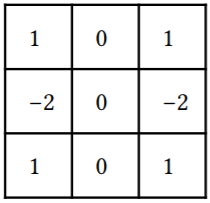
\includegraphics[width=1in]{gradient_filter.png}
        \caption{Pixel region where numbers indicate brightness of the pixel}
        \label{gradfilter}
\end{figure}

\begin{figure}
        \centering
        \subfloat[]{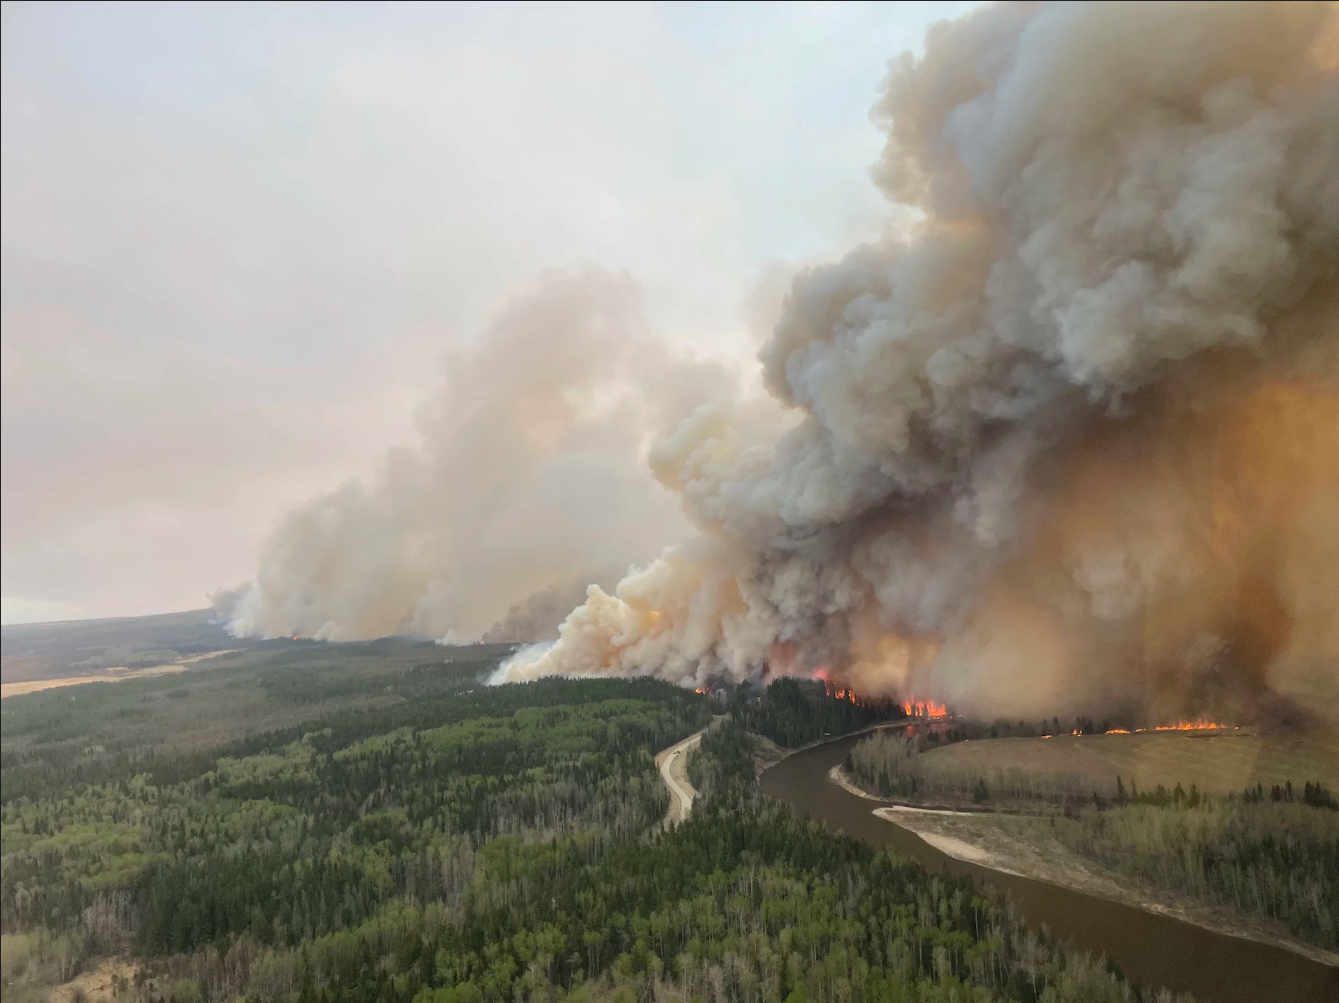
\includegraphics[width=2in]{sobel_original.png}%
        \label{sobel_orig}}
        \hfil
        \subfloat[]{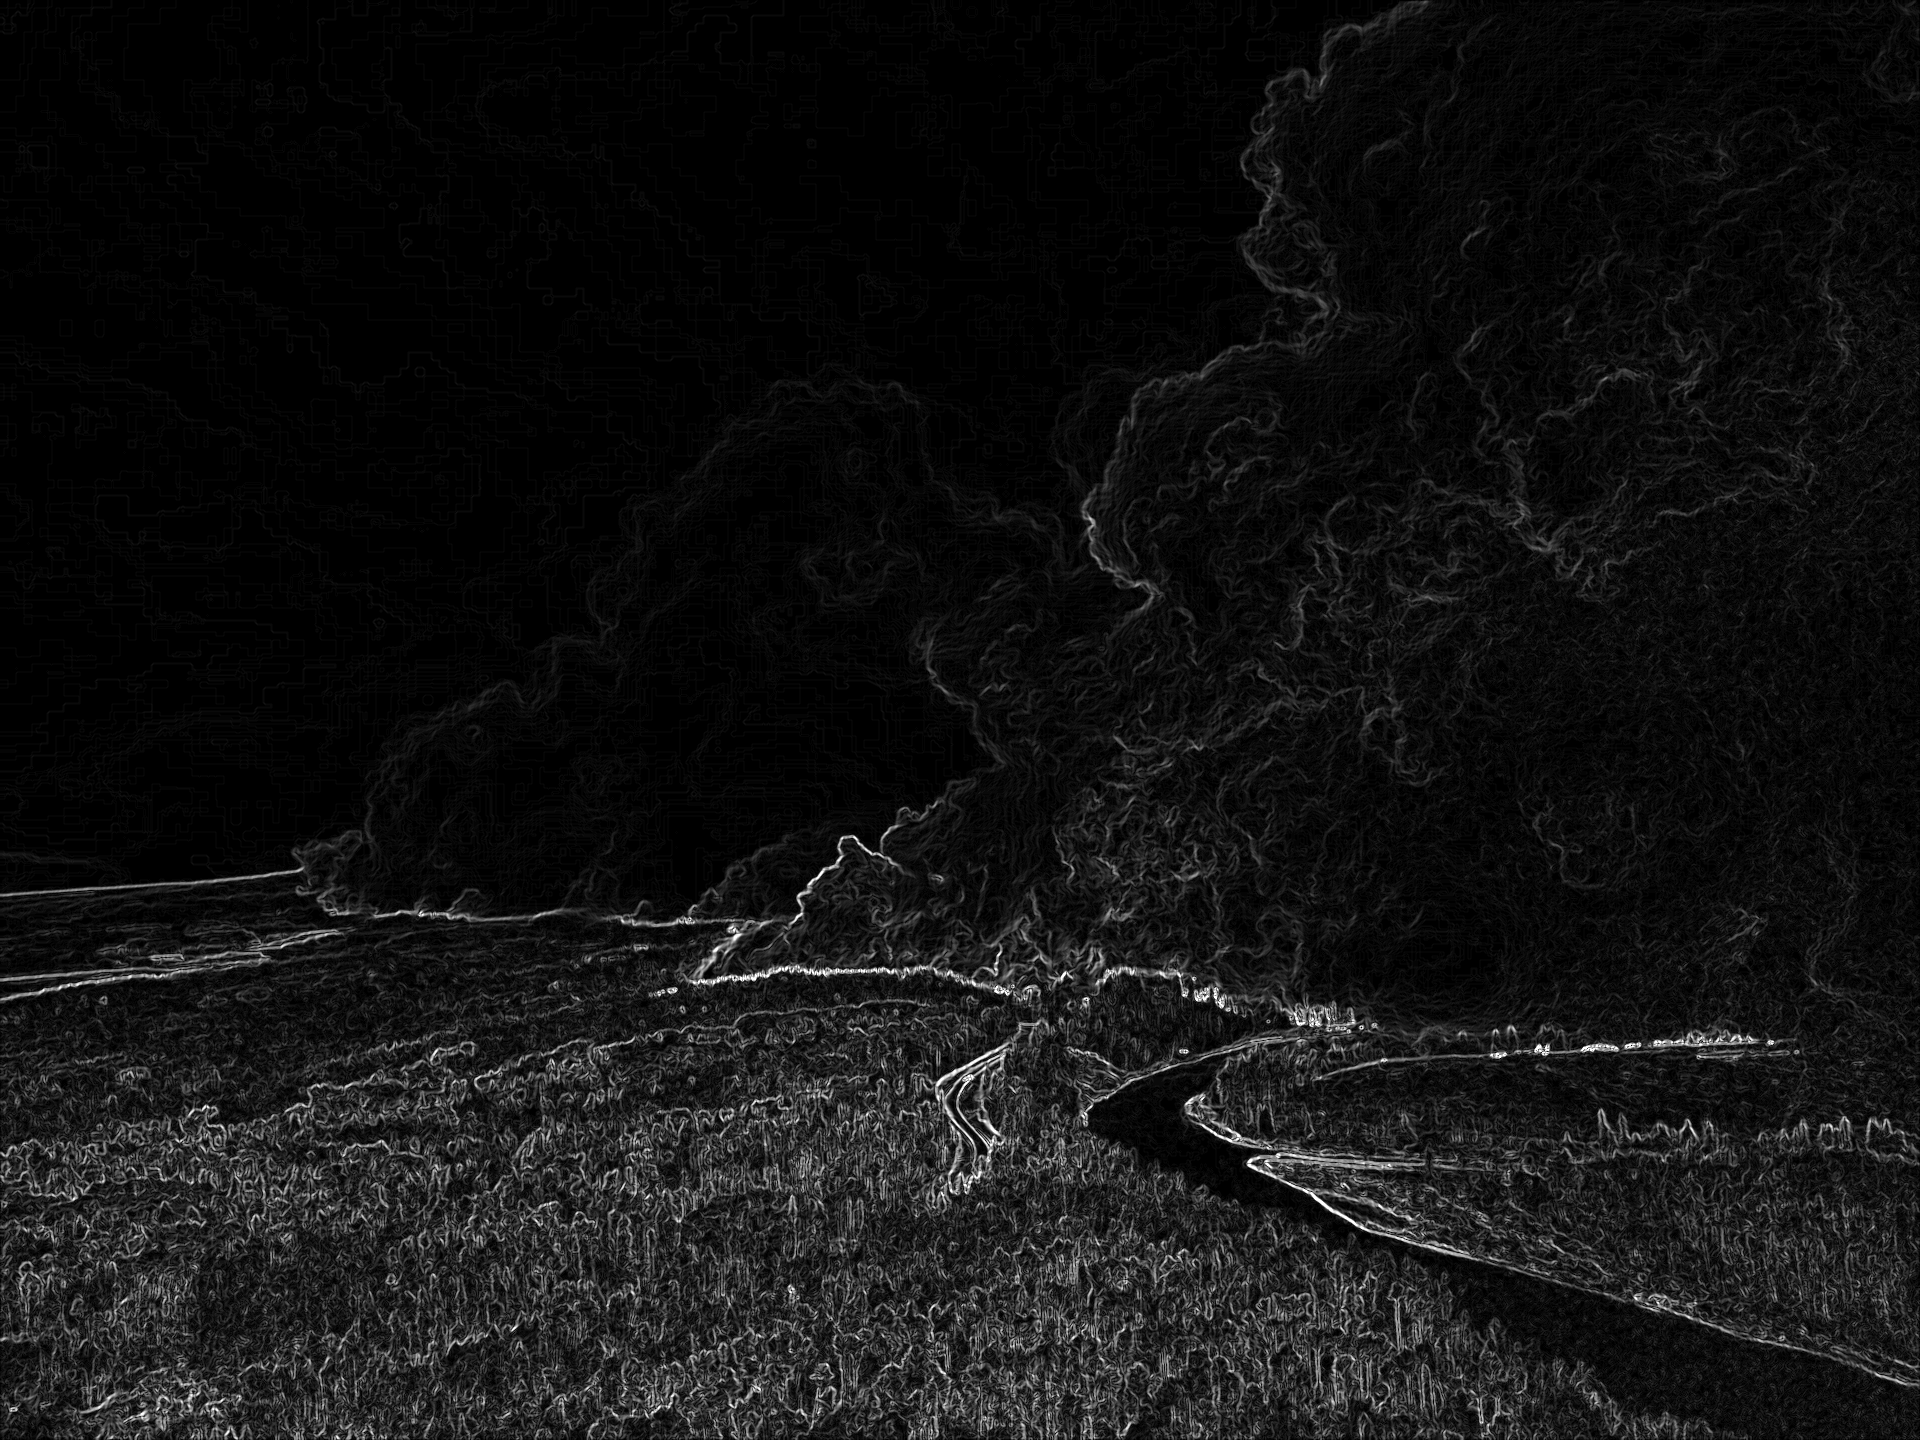
\includegraphics[width=2in]{sobel.png}%
        \label{sobel_filter}}
        \caption{Image with smoke processed using a basic sobel filter}
        \label{sobelimg}
\end{figure}

\subsubsection{Corner Detection}

Corner detection is a common technique used in computer vision to infer
features from an image. \cite{prepfire} shows that a corner detection
algorithm is a vital preprocessing stage, as it separates fire from
other objects of similar color, which would fall within the thresholds
of a HSV filter. The popular Harris corner detector uses the
autocorrelation function of the image to determine intensity differences
within patches of an image. Using a Taylor expansion, the
autocorrelation function can be approximated as
\cite{prepfire}\cite{harriscorner}:

\[I\left( x_{i},y_{i} \right) + \left\lbrack I_{x\left( x_{i},y_{i} \right)}I_{y\left( x_{i},y_{i} \right)} \right\rbrack\begin{pmatrix}
u \\
v
\end{pmatrix}\]

Where \(I\) represents intensity and \(u\) and \(v\) represent the shift
in the region from the reference pixel \(\left( x_{i},y_{i} \right)\).
This shows that the change in intensity depends on the partial
derivatives \(I_{x}\) and \(I_{y}\) of the image. When written in matrix
form, the expression is as follows:

\[M = \begin{pmatrix}
\sum(I_{x\left( x_{i},y_{i} \right)}^{2}) & \sum(I_{x\left( x_{i},y_{i} \right)}I_{y\left( x_{i},y_{i} \right)}) \\
\sum(I_{x\left( x_{i},y_{i} \right)}I_{y\left( x_{i},y_{i} \right)}) & \sum(I_{y\left( x_{i},y_{i} \right)})
\end{pmatrix}\]

The eigenvalues of the matrix can be found using the determinant and
trace:

\[\text{ det}(M) = AB - C^{2} = \lambda_{1}\lambda_{2}\]
\[\text{ trace}(M) = A + B = \lambda_{1} + \lambda_{2}\]

There are three possible situations based on their values:

\begin{itemize}
\item
  Both eigenvalues are small: this happens when the pixels are in a flat
  region
\item
  One eigenvalue is bigger than the other eigenvalue: The region likely
  is an edge
\item
  Both eigenvalues are large: the region is a corner
\end{itemize}

Therefore, corner regions within an image will output a high corner
strength. These regions can be used as a candidate region that can be
inferred through a CNN.

\begin{figure}
        \centering
        \includegraphics[width=2in]{corner.png}
        \caption{Corner detection executed on HSV-filtered image of fire
        (corners marked green)}
        \label{corner}
\end{figure}

\subsubsection{Dark Channel Prior}

Dark Channel Prior has been commonly used to measure the degree of
haziness as well as haze-removal in images. The technique is based on
the observation that in most outdoor images, pixels tend to have low
intensities in atleast one colour channel (dark channel). This property
can be used to estimate the transmission map of an image, representing
the amount of haze affecting the scene. Atmospheric haze can be modelled
as follows \cite{darkchannelprior}:

\[I(x) = J(x)t(x) + A\left( 1 - t(x) \right)\]

\(I(x)\) represents a pixel that reached the camera. \(J(x)\) represents
the undistorted pixel. \(t(x)\) is the transmission map, representing
how much scene radiance is retained, where a value of 1 means no haze
and 0 means maximum haze. Due to the scattering of light from haze, low
intensity channels in hazy patches of an image have an inherently higher
value. As a result, DCP can be used to estimate \(t(x)\) providing the
areas of the image affected by haze. \cite{prepfire} and \cite{dcpsmoke}
note that dark channel prior methods can apply to smoke due to the
similar nature, having relatively higher values in their dark channels.
This causes smoke to be picked up as an area of high haze in the
transmission map. \cite{prepfire} apply a threshold to the transmission
map, extracting areas with high dark channel values and suppressing the
rest. As a result, a 6\% increase in detection accuracy was achieved
compared to detection without extra preprocessing stages.

As shown in figure \ref{dcp}, DCP reveals areas with high
intensity values in all three channels, causing haze, smoke, and sky
regions to appear very bright compared to the rest in the second image.
In the third image, regions below a certain intensity threshold are
suppressed to zero. This gives us the regions where there is a high
chance of smoke or fog.

Despite the notable improvements in smoke detection using dark channel
prior, there are some drawbacks to be considered. Dark channel prior
tends to be unreliable when the image consists of a large portion of
sky, since the sky tends to have a high dark channel value, causing the
algorithm to mistake it as hazy or smoky area. This is evident in
figure \ref{dcp}, where the sky is included in the final
thresholded output image.

\begin{figure}
        \centering
        \subfloat[]{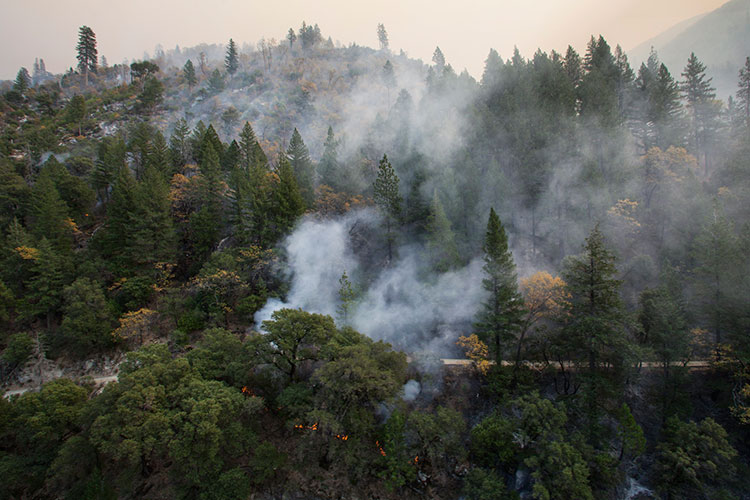
\includegraphics[width=2in]{WildfireSmoke.jpeg}%
        \label{dcp_orig_img}}
        \hfil
        \subfloat[]{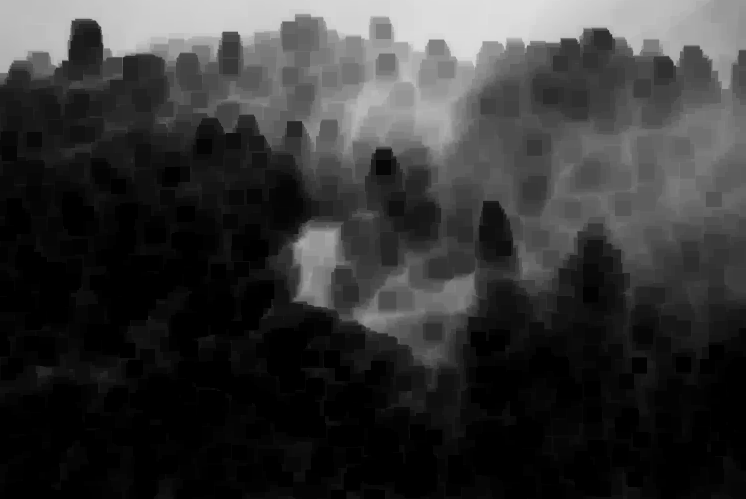
\includegraphics[width=2in]{dcp_original.png}%
        \label{dcp_orig}}
        \caption{Image processed with Dark channel prior \& thresholded to high
        intensity values (a) Original image (b) Dark channel processed image}
        \label{dcp}
\end{figure}

\subsubsection{Histogram Equalization}

Histogram Equalization increases the global contrast in images, which
can enhance the visibility of finer details within an image. The
algorithm spreads the intensity values out in an image so that it
utilizes the full range of values more efficiently \cite{he}. As a
result, HE is most effective on images with a narrow range of intensity
values.

HE's effectiveness at enhancing image quality makes it a practical
technique in many scenarios. \cite{shipfirehe} presents a system to
detect early fires inside a ship using a YOLO computer vision model.
Images were preprocessed with Histogram Equalization to reduce the
impact of water vapour on the quality of the images, contributing to the
remarkable 99\% accuracy of the model. \cite{xrayhe} investigates using
CLAHE, an advanced form of histogram equalization along with a YOLOv4
model to detect bone fracture features in xray images, obtaining a
result of 81.91\% when trained on a small dataset.

Let us consider \(n_{i}\) as the number of occurences of the gray level
\(i\) in a greyscale image. The probability of a pixel with level \(i\)
is as follows:

\[p(i) = \frac{n_{i}}{n},0 \leq i < L\]

Where \(L\) is the total number of gray levels in the image. The
cumulative distribution function can then be defined:

\[\text{ cdf}(i) = \sum_{j = 0}^{L}p(j)\]

In order to achieve a flat histogram of values, the CDF must be
linearized. This can be carried out by the following equation:

\[h(v) = \text{ round}\left( \frac{\text{cdf}(v) - \text{ cdf}_{\text{min}}}{N - \text{ cdf}_{\min}} \right)\]

Where \(N\) is the number of pixels in the image.

By applying this function to each pixel of the original image, we obtain
a resulting image with a flatter histogram of intensities, increasing
contrast and visibility in the image. An example of this contrast enhancement in shown in figure \ref{heq}.

\begin{figure}
        \centering
        \subfloat[]{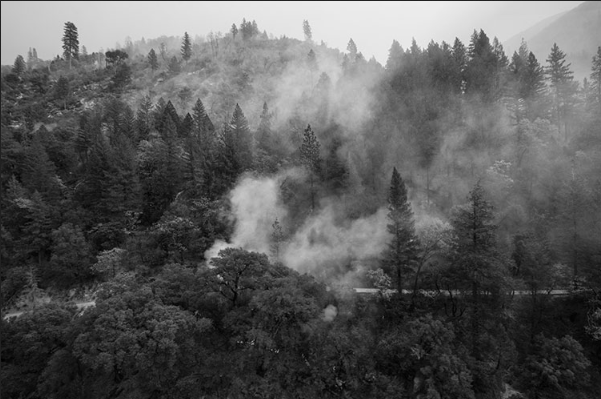
\includegraphics[width=2in]{he_original.png}%
        \label{he_orig}}
        \hfil
        \subfloat[]{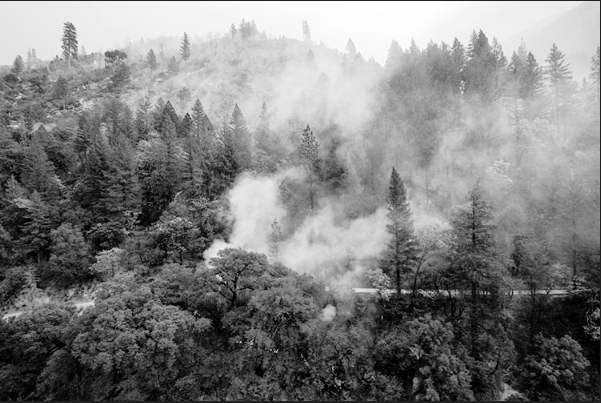
\includegraphics[width=2in]{he_processed.png}%
        \label{he_processed}}
        \caption{Histogram equalization on image}
        \label{heq}
\end{figure}

\section{An Improved Smoke Detection System}

Using Dark Channel Prior to preprocess images has proven to be
worthwhile for improving detection accuracy
\cite{dcpsmoke}\cite{dcpsmoke2}. By isolating smoke areas from other
background noise in the image, DCP simplifies classification for a
neural network, allowing for better results on smaller datasets and
shallower, faster models. However, DCP fails to be effective in images
that contain other artifacts of high light-intensity, such as the sky.
This could cause inconsistent results particularly in terrestrially
placed detection nodes, where the camera might have small parts of the
sky in frame.

Generally, we can assume that smoke in an image is more noisy and
contains contours and textures that a plain sky would not have. This
texture can be picked up by a Sobel operator in an edge response image.
The response image may be used to identify areas with very little edge
response which can safely be eliminated from consideration.

In order to eliminate certain areas of an image from being considered in
the DCP algorithm, a binary threshold can be used on the image, which
will either suppress pixels to zero or change them to max value
depending on a thresholding condition. This can be useful for creating a
map of unwanted sections in an image that can be suppressed at a later
stage. We can provide the Sobel filtered image to a binary threshold to
supress only parts of the image which have an edge response very close
to 0. The resulting image mask would be black in sky areas, allowing us
to effectively detect sky regions.

In figures \ref{sobelsky} and \ref{edgedcp}, A sobel filter as well as dark
channel prior image is computed from the original image. The edge
response image is generously dilated and blurred in order to mitigate
small dark spots in the image as they are irrelevant. After applying a
binary threshold, this image is used on the DCP output to suppress the
pixel regions of sky.

\section{Drawbacks}

The proposed Sobel/DCP method eliminates sky regions from an image in most cases.
However the performance may be inconsistent in certain conditions such as cloudy skies or the presence of black smoke.
In certain situations where the sky is partially cloudy, clouds may take up a similar shape and texture to early wildfire smoke, scattering light in a similar way causing the algorithm to classify it as a positive region for the existence of smoke. 
Black smoke, usually associated with the combustion of fuels is missed by the algorithm as it's dark channel light intensity falls lower than the algorithm's threshold. 

The Sobel/DCP algorithm's downsides indicates effectiveness specifically at white or light gray smoke. Darker smokes have the propensity to have light intensities that are too low for the algorithm to notice. Studies have linked light gray and white smoke with smouldering fires or those in early stages \cite{smokecolour}. The proposed algorithm could prove to be useful at early wildfire detection, allowing a wildfire response team to be notified faster, potentially preventing a larger disaster.

% need images..

\section{Experimental Results}

The dark channel edge detection system was tested on various images as
well as on a large smoke \& fire dataset to benchmark speed \&
computational intensity, which are important in edge computing systems.
The tested images show that the algorithm effectively separated smoke
from sky and other unwanted noise, also being able to suppress the image
completely in cases of no detected smoke or haze.

Notable weak points of the algorithm include differentiation between
smoke and clouds. Smaller clouds with visible edges and contours can
appear similar, which may reduce the algorithm's accuracy. Darker smoke
such as those from burning fossil fuels are not easily detected by the
edge + dcp algorithm. Since dark channel prior favours high light
intensity values, dark gray or black smoke does not have any
characteristics that DCP can detect.

\begin{figure}
        \centering
        \includegraphics[width=2in]{sobelsky.png}
        \caption{The sobel edge filter has close to zero response on sky
        regions}
        \label{sobelsky}
\end{figure}

\begin{figure}
        \centering
        \subfloat[]{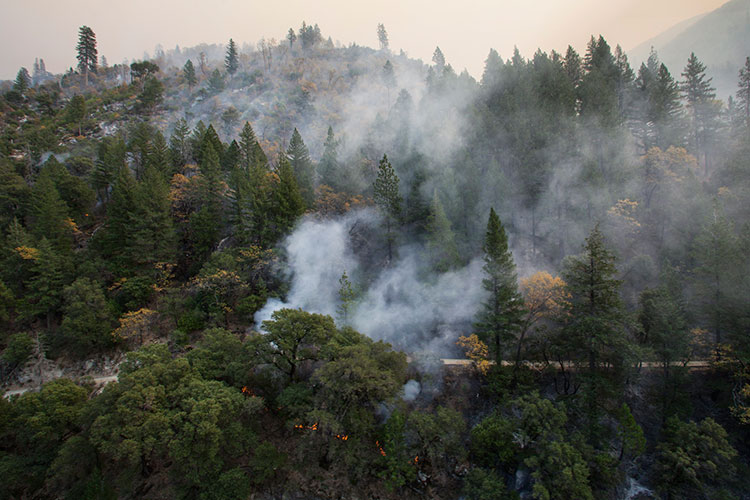
\includegraphics[width=2in]{WildfireSmoke.jpeg}%
        \label{edcp_orig}}
        \hfil
        \subfloat[]{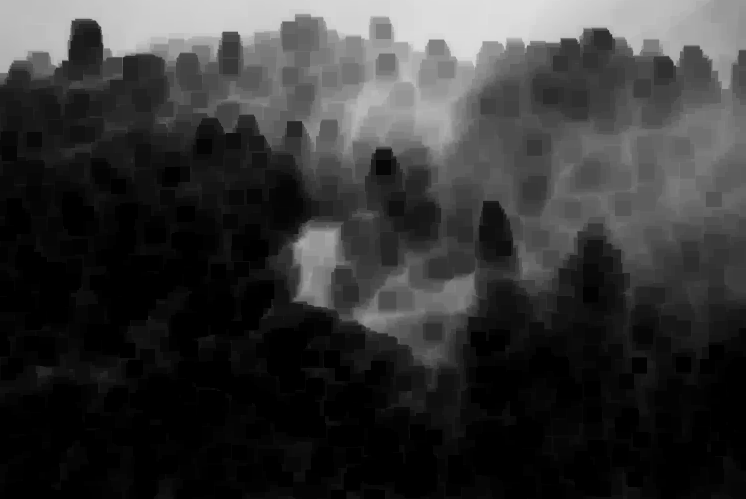
\includegraphics[width=2in]{dcp_original.png}%
        \label{edcp_b}}
        \hfil
        \subfloat[]{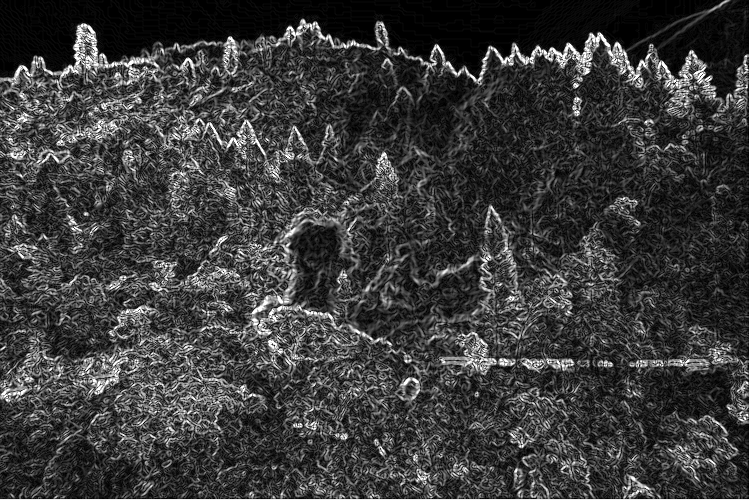
\includegraphics[width=2in]{edcp_sobel.png}%
        \label{edcp_c}}
        \hfil
        \subfloat[]{
\includegraphics[width=2in]{edcp_skyfilter.png}%
        \label{edcp_d}}
        \hfil
        \subfloat[]{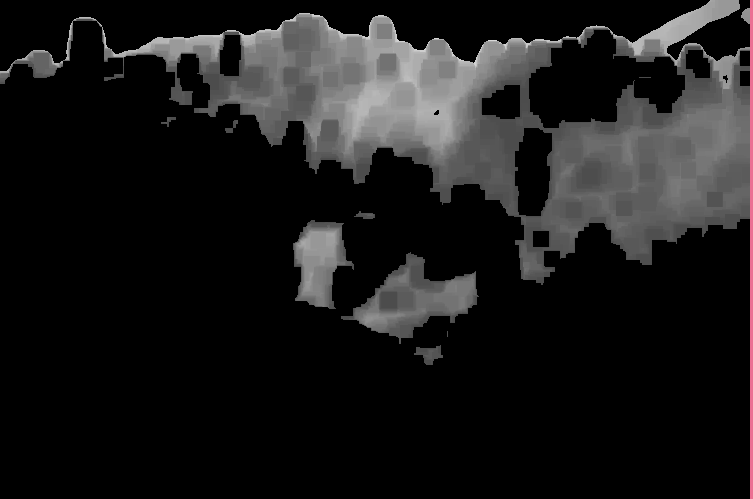
\includegraphics[width=2in]{edcp.png}%
        \label{edcp_e}}
        \caption{Edge Detection \& DCP Filtering to detect smoke without
        conflating sky regions (a) Original image. (b) DCP processed image. (c) Sobel filtered image. (d) Sky filter by dilating the sobel output. (e) Thresholded DCP image combined with sky filter, leaving only smoke regions.}
        \label{edgedcp}
\end{figure}


\bibliographystyle{IEEEtran}
\bibliography{ref}

\newpage


\vfill

\end{document}


